Macroscopic and microscopic approaches are used for measuring \glspl{DNP} \cite{parish1999status, rudstam2002delayed}.
%There are two approaches used for measurement of \glspl{DNP}, referred to as the macroscopic and microscopic measurement approaches \cite{parish1999status, rudstam2002delayed}.
The macroscopic approach, discussed in detail in Section \ref{sec:macro-eval}, uses a fissile sample irradiation to get the delayed neutron count rate, which can be approximated using groups.
%The approaches differ initially, as the macroscopic approach uses a fissile sample irradiation to get delayed neutron counts which can be approximated using groups.
Conversely, the microscopic approach, discussed in detail in Section \ref{sec:micro-eval}, uses the data from many experiments combined together to simulate a fissile sample irradiation and generate the delayed neutron count rate.
The microscopic approach is more challenging, as it depends on the work of many experimentalists.
However, it offers more detail on the delayed neutron count rate.

\subsubsection{Macroscopic Measurement of DNPs}
\label{sec:macro-eval}
The macroscopic approach entails irradiating a sample containing a single fissile nuclide at or near a given neutron energy.
This delayed neutron count rate from this sample can then be measured and used to formulate \gls{DNP} group parameters.
Analysis and collection of macroscopic experiment data is common in the literature \cite{keepin1957delayed, tuttle1975delayed, manero1972status, benedetti1982delayed, waldo1981delayed, brady1988evaluation, hughes1948delayed, loaiza1998measurements, loaiza2000dominant, conant1971measurement}.

Small samples are used to minimize neutron multiplication within the sample to avoid spectral effects \cite{keepin1957delayed}.
The spectral effects are due to the differing neutron energy spectra between each \gls{DNP} group and the incident irradiating neutrons \cite{keepin1957delayed}.
Another reason for using a small sample is because of physical challenges associated with the rabbit system \cite{brunson1955measurement}.

Two different types of irradiation are used: pulse and infinite. 
Pulse irradiation has an irradiation time shorter than the shortest half-life, and it captures the shorter lived \glspl{DNP} with more accuracy than the longer lived \glspl{DNP} \cite{brady1988evaluation}.
Infinite irradiation has an irradiation time longer than several times the longest half-life, and it captures the longer lived \glspl{DNP} with more accuracy than the shorter lived \glspl{DNP} \cite{brady1988evaluation}.
After irradiation, the delayed neutrons from the sample are counted as a function of time.
The delayed neutron count rate as a function of time after irradiation, $n_d(t)$, is given as:

\begin{equation}
    \dot{n}_d(t) = \epsilon \sum_{i=1}^{I} P_{n, i} \lambda_i N_{i}(t),
    \label{eq:mdnp-dn}
\end{equation}
where,
\begin{align}
\dot{n}_d(t) &= \mbox{ the delayed neutron count rate $\left[\frac{n}{s}\right]$ }\nonumber \\
I &= \mbox{ the total number of \glspl{DNP} [-] } \nonumber \\
\epsilon &= \mbox{ the detector efficiency [-].} \nonumber
\end{align}

%\begin{description}
%    %\setlength\itemsep{-0.25em}
%    \item $I$ is the total number of \glspl{DNP}
%    \item $\epsilon$ is the detector efficiency
%\end{description}

Once this delayed neutron count rate is generated, the data is used to generate \gls{DNP} group and kinetics parameters for that fissile nuclide and neutron energy.
Three different approaches have been used to generate \gls{DNP} group parameters from macroscopic data: exponential stripping (or peeling) \cite{brunson1955measurement, keepin1955delayed}, least-squares \cite{brady1988evaluation, keepin1957delayed}, and using half-lives of specific \glspl{DNP} \cite{saphier1977evaluated}.
Some approaches have even used a combination, such as least-squares fitting with specific half-lives \cite{spriggs20028}.
The exponential stripping, or peeling, method is essentially a more subjective form of least-squares fitting, where exponential curves are subtracted away from the raw data from right to left \cite{price2020review}.
The use of specific half-lives to form the \gls{DNP} groups is less subjective and offers a more physical interpretation of the groups.
The least-squares approaches are the most objective approach and generate groups which physically do not embody a single \gls{DNP}.
Instead, they group together the \glspl{DNP} and effectively capture the overall physical effect, minimizing the objective function.
For this work, the least-squares approach is used, as it offers an objective formulation that can be generically applied.
%The specifics of the methods used to form those parameters is discussed in Section \ref{sec:gandkparams}.
The specifics of the least-squares approach used to form the \gls{DNP} parameters is discussed in Section \ref{sec:calc-group-param}.
Figure \ref{fig:keepin-setup} (recreated from \cite{keepin1957delayed}) shows an experimental setup for collecting delayed neutrons.

%\begin{figure}[H]
%    \centering
%    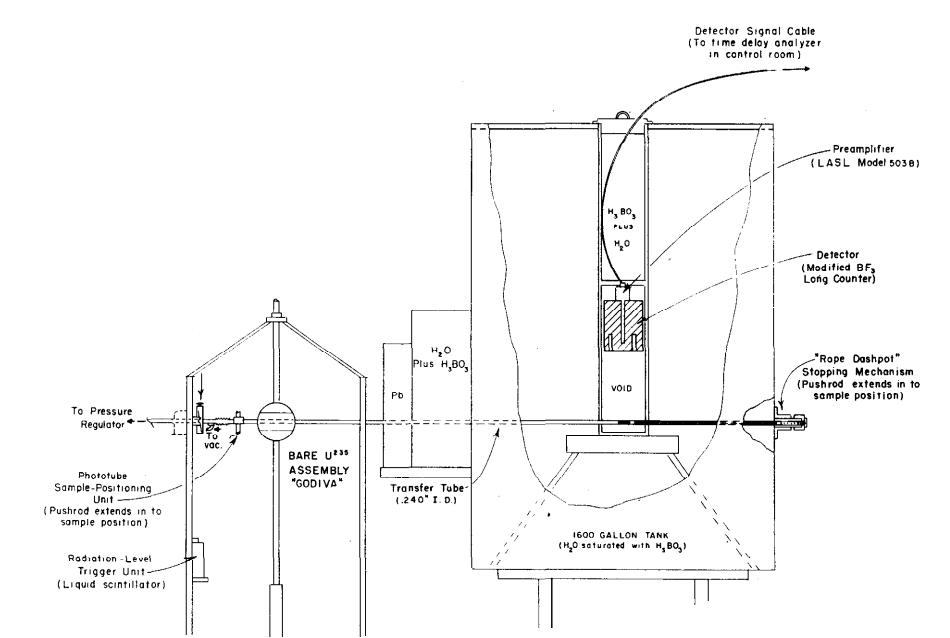
\includegraphics[width=0.80\linewidth]{images/keepin-setup.PNG}
%    \caption{Experimental setup for measuring delayed neutron emission from irradiation of a 3 gram sample in %Godiva recreated from \cite{keepin1957delayed}.}
%    \label{fig:keepin-setup}
%\end{figure}

\begin{figure}[H]
    \centering
    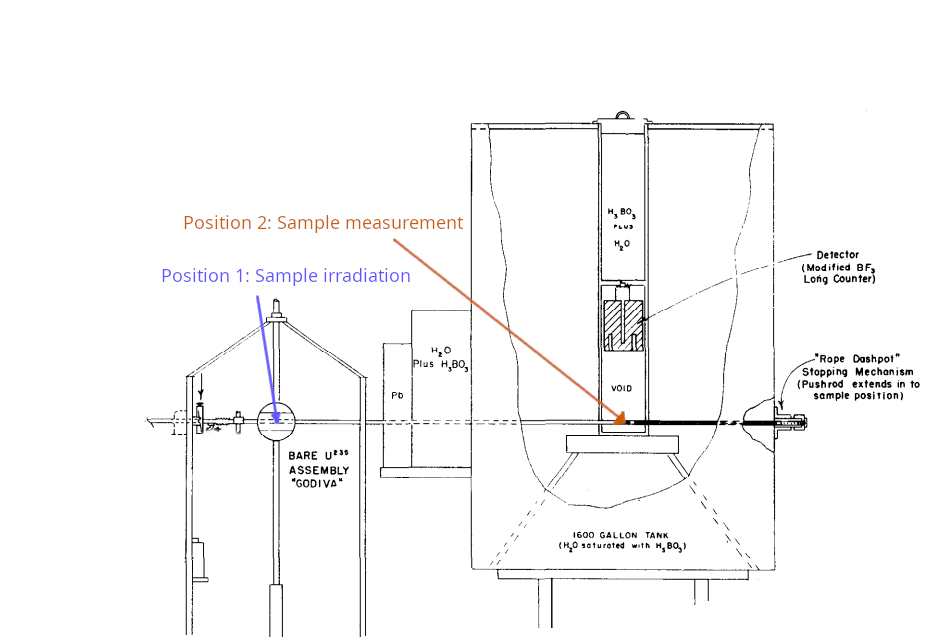
\includegraphics[width=0.80\linewidth]{images/keepin-setup-mod.png}
    \caption{Simplified experimental setup for measuring delayed neutron emission from irradiation of a 3 gram sample in Godiva referenced from \cite{keepin1957delayed}.}
    \label{fig:keepin-setup}
\end{figure}

Challenges associated collecting this experimental data \cite{bank2000jef} include experimental noise and signal obfuscation due to moderation. 
Experimental noise becomes significant after long periods of time relative to the half-life of the longest-lived \gls{DNP}, around 1 minute from $^{87}$Br, as the delayed neutron counts decrease.
Additionally, the short lived groups cannot be measured directly due to moderated neutrons from irradiation, so there is a gap between irradiation and when the sample can be moved to a delayed neutron counter.
Even after a pulse irradiation, the long-lived groups form a background that interfere with measurement of the short-lived groups \cite{bank2000jef}.
Due to these effects, measurement of delayed neutrons from the sample is less accurate initially, becomes increasingly accurate, and then becomes less accurate again as the delayed neutron counts decrease.

Similarly, uncertainty arises from the measurement of the number of fissions.
Although the number of fission events can be measured somewhat accurately using a fission chamber after irradiation or other techniques, the fission chamber does not account for source multiplication within the irradiated sample.
Keepin et al. suggests a technique to correct for the sample self-multiplication.
The sample self-multiplication require a correction factor of up to 3\% in the number of fissions.

\subsubsection{Microscopic Measurement of DNPs}
\label{sec:micro-eval}
The other approach used to measure \glspl{DNP} is the microscopic -- also referred to in the literature as the aggregate or summation -- approach, which uses data from individual nuclides summed together to form a simulated delayed neutron count rate.
This count rate can then be used to generate \gls{DNP} group parameters, the same as in the count rate from the macroscopic method.
This approach was investigated in detail in the 1990-2000's \cite{pfeiffer2002status, d2002review, rudstam2002delayed, wilson2002delayed, brady1989delayed}, with progress through the 2010's with more data \cite{mills2014calculation, huynh2014calculation}. Leconte et al. used this approach as recently as 2020 \cite{leconte2020new}.
This approach requires experiments on individual \gls{DNP} nuclides, from which emission probabilities and half-lives can be measured.
Typically, this involves rapid chemical extraction or isotope separation and magnetic tape to rapidly measure short lived nuclides, such as in the study by Björnstad et al. where an aluminized mylar tape is used \cite{bjornstad1981decay}.
The magnetic tape is used to transport samples or remove longer-lived decay products \cite{shalev1974energy, rudstam1974delayed}.
Experimental methods include the neutron-$\beta$ coincidence technique, separate counting of neutrons and $\beta$ particles, separate counting of neutrons and $\gamma$ rays, ion counting, fission yield from a set number of fissions, gamma counting of a long-lived daughter, and normalization of the neutron counter using a known precursor \cite{rudstam1974delayed}.

Other experimental methods used to study \glspl{DNP} include on-line mass spectrometry, helium-3 spectrometry, proton-recoil detectors, the time-of-flight method, and neutron scintillators \cite{das1993importance}.
On-line mass spectrometry combined with a helium-3 ionization chamber and a proton-recoil detector allows for measurement of the delayed neutron energy spectrum \cite{shalev1972delayed, beyer2007proton}.   
The time-of-flight technique consists of measuring the flight time of a neutron over a known distance to calculate the velocity, including a neutron scintillator \cite{beyer2007proton, chulick1971energy, garcia2012monster, chrysochoides1971measurement}.
\begin{comment}
An example of the time-of-flight experimental setup is shown in Figure \ref{fig:micromeasure}.

\begin{figure}[H]
    \centering
    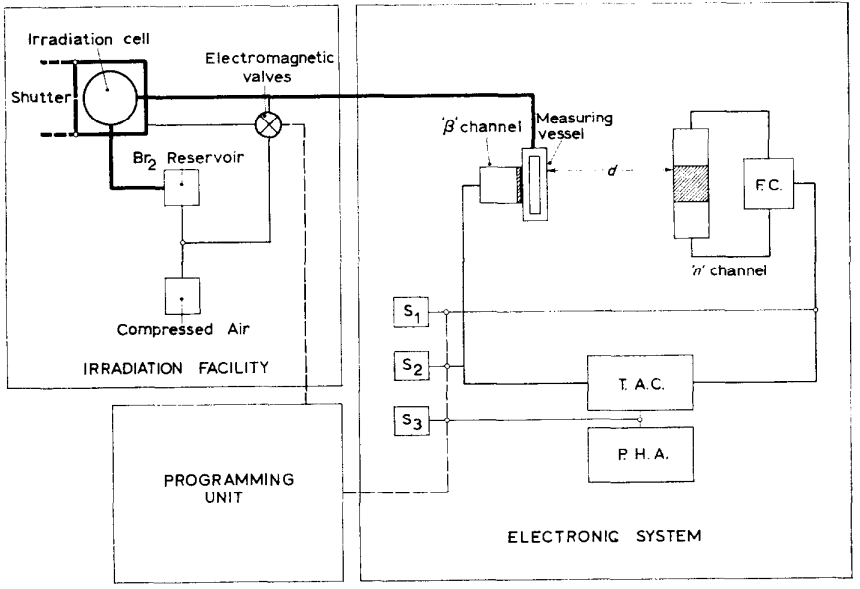
\includegraphics[width=0.80\linewidth]{images/micromeasure.PNG}
    \caption{A block diagram of the time-of-flight experimental setup for measuring delayed neutrons from bromine-87 and bromine-88, extracted from the Democritos reactor via a fast radiochemical technique recreated from  \cite{chrysochoides1971measurement}.}
    \label{fig:micromeasure}
\end{figure}
\end{comment}

This microscopic measurement data is exceptionally useful, as it allows for treatment of \glspl{DNP} on a nuclide-by-nuclide basis.
This is particularly important for \glspl{MSR}, where the spatial \gls{DNP} concentration depends on half-lives, yields, thermo-chemistry, and thermal-hydraulics.
With data on individual nuclides, higher fidelity treatment of \glspl{DNP} becomes possible.

There have been many new measurements in the past several decades on these nuclides.
The \gls{IAEA} has compiled and evaluated this data in a publicly accessible form \cite{DIMITRIOU2021144, dillmann2015summary}.
This data, when combined with cumulative fission yields and neutronics data, can be used to model the \glspl{DNP} explicitly rather than using groups.
This is particularly useful for understanding what nuclides have the greatest impact, as well as for simulating experimental configurations which have yet to be thoroughly investigated for \gls{DNP} group fitting.